\documentclass[11pt]{article}
\usepackage[margin=1in]{geometry}
\usepackage{graphicx}
\usepackage{lmodern}
\usepackage{pdflscape}
\usepackage{longtable,booktabs,array}
\usepackage{tikz}
\usetikzlibrary{arrows.meta,calc,fit,backgrounds}

\title{HW1 Design Report\\\large COMS E6998-019: Design of Production Agentic Systems}
\author{}
\date{}

\setlength{\parindent}{0pt}

\usepackage{url}
\begin{document}
\maketitle

\section*{Part A: Design report}
\subsection*{A1. Behavioural contract}

\noindent\textbf{Purpose and scope}\par\smallskip
The agent classifies one Bandit alert at a time in a pinned Python checkout. It determines whether the reported pattern represents a real security issue, returning label 1 or 0 with code evidence when it can classify; otherwise it produces a controlled null-label error or cutoff row. Bandit discovery is separate from model investigation: Bandit discovers the in-scope MEDIUM+ alerts, while the model investigates each discovered alert using only approved read-only tools.

\vspace{6pt}
\noindent\textbf{Normal per-alert behaviour}\par\smallskip
\begin{enumerate}
  \item The runner discovers and sorts Bandit alerts.
  \item For one alert, it creates a disposable agent workspace.
  \item The controller receives the alert and initial instructions.
  \item The model either requests repository investigation tools or submits JSON.
  \item The dispatcher validates every tool request, runs approved requests, and returns the actual observation.
  \item The model may use those observations for another decision.
  \item A valid submission becomes one classified report row with rationale and evidence.
  \item The runner proceeds to the next alert.
\end{enumerate}

\medskip
\noindent\textbf{Safety and observational integrity}\par\smallskip
\begin{itemize}
  \item The agent must never execute code from the target repository.
  \item The agent must never modify the target repository, including by writing, editing, patching, or deleting files.
  \item The agent must never fabricate file contents, command results, tool observations, or evidence ranges.
  \item The agent must never allow the model to read outside its disposable workspace or access \texttt{.git}.
  \item On OWASP BenchmarkPython, the agent must never expose the answer key or any sibling \texttt{BenchmarkTest*} case.
\end{itemize}
The model proposes a tool request. The runtime/dispatcher validates and executes it. Only the dispatcher writes tool observations into the trace.

\par\medskip\noindent\textbf{Controlled outcomes}\par\smallskip
The system does not silently drop alerts. A malformed submission becomes an error row for that alert, and a denied tool request becomes a refusal observation rather than a crash. A budget cutoff, max-step cutoff, or no-progress stop ends the active run under runtime control. The runner still writes one row for every discovered alert.

\clearpage
\begin{landscape}
\subsection*{A2. State machine}
\begin{center}
\resizebox{0.98\textwidth}{!}{%
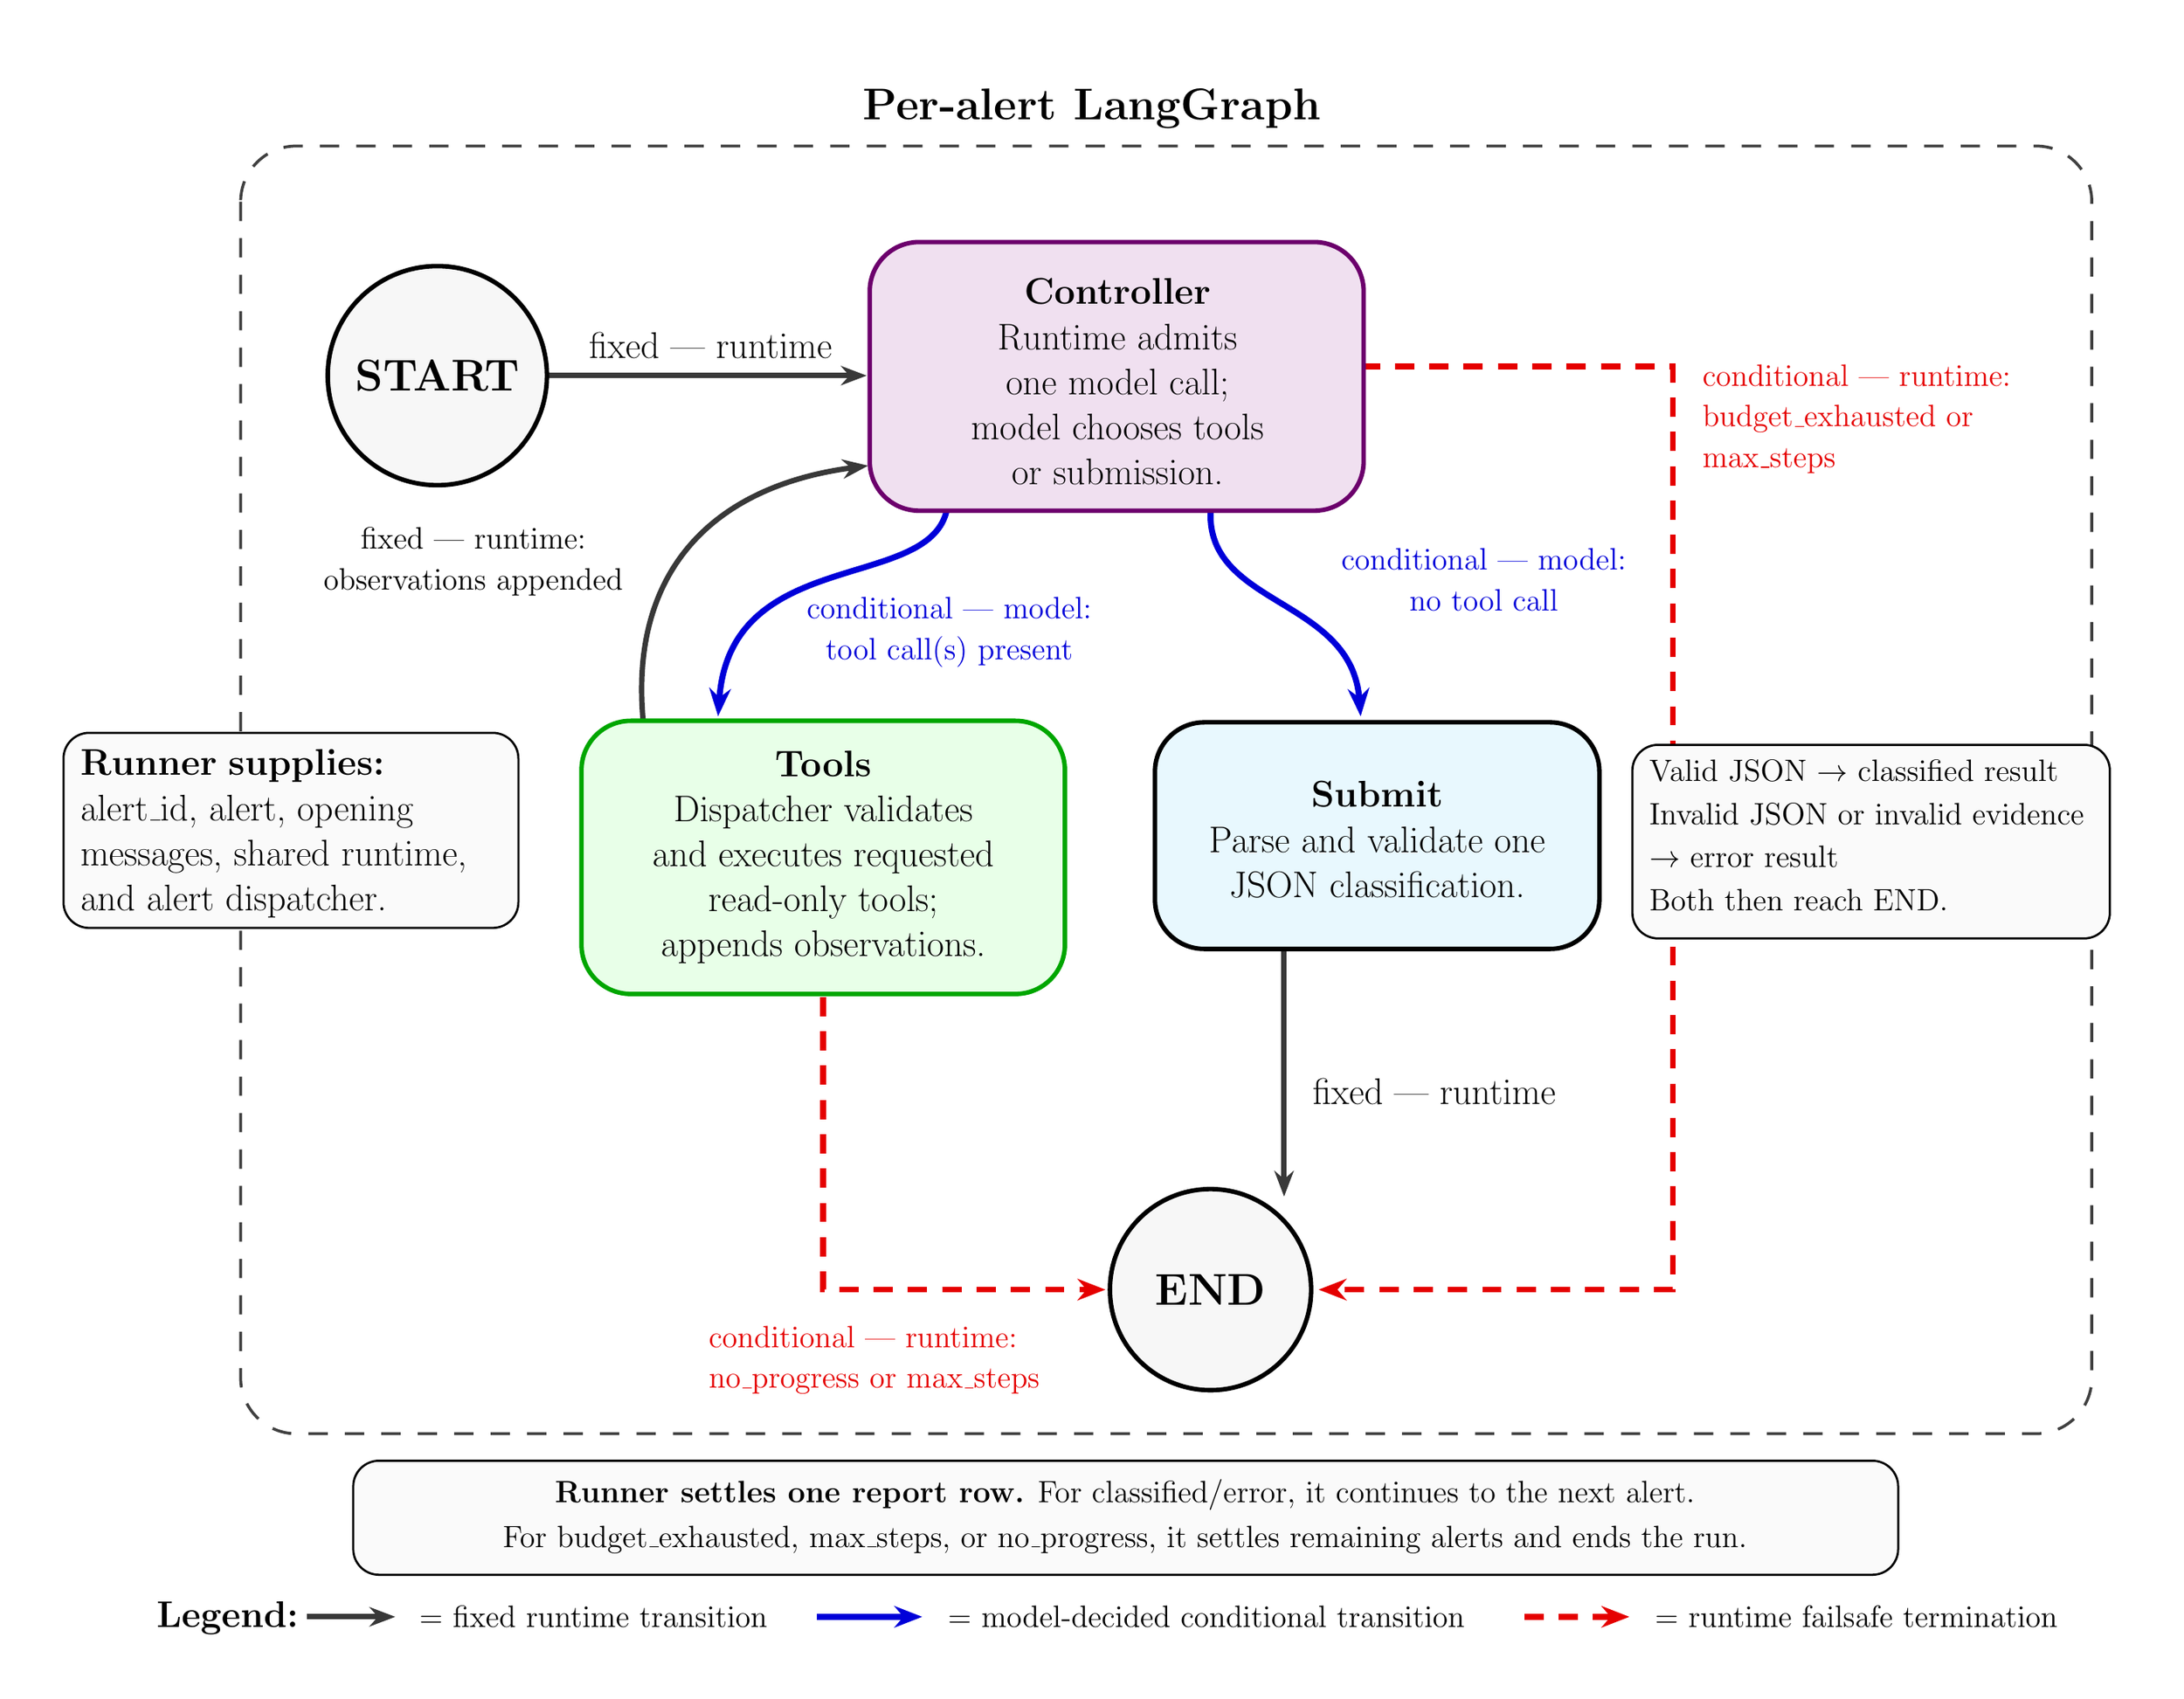
\begin{tikzpicture}[x=.70pt,y=-.70pt,>=Stealth,
 box/.style={rounded corners=23pt,line width=2.1pt},
 fixed/.style={draw=black!78,line width=2.5pt,-{Stealth[length=12pt,width=9pt]}},
 model/.style={draw=blue!85!black,line width=2.8pt,-{Stealth[length=13pt,width=10pt]}},
 fail/.style={draw=red!90!black,line width=2.8pt,dash pattern=on 9pt off 7pt,-{Stealth[length=13pt,width=10pt]}},
 copy/.style={font=\fontsize{17}{21}\selectfont,align=center,inner sep=0pt},
 smallcopy/.style={font=\fontsize{15}{19}\selectfont,align=center,inner sep=0pt}]
\path[use as bounding box] (0,0) rectangle (1426,1103);
\draw[black!75,line width=1.35pt,dash pattern=on 9pt off 8pt,rounded corners=26pt] (146,83) rectangle (1379,941);
\node[font=\bfseries\fontsize{21}{24}\selectfont,fill=white,inner xsep=10pt] at (713,58) {Per-alert LangGraph};

\draw[fixed] (349,236)--(563,236);
\draw[fixed] (414,465) .. controls (405,363) and (464,309) .. (564,296);
\draw[model] (616,327) .. controls (602,380) and (472,350) .. (464,463);
\draw[model] (792,327) .. controls (790,390) and (886,384) .. (892,463);
\draw[fixed] (841,619)--(841,783);
\draw[fail] (892,230)--(1100,230)--(1100,845)--(864,845);
\draw[fail] (534,650)--(534,845)--(722,845);

\draw[black,line width=2.1pt,fill=black!3] (277,236) circle[radius=73];
\node[font=\bfseries\fontsize{21}{25}\selectfont] at (277,236) {START};
\draw[box,draw=violet!85!black,fill=violet!12] (565,147) rectangle (894,326);
\node[copy,text width=310pt] at (730,240) {\textbf{Controller}\\ Runtime admits\\ one model call;\\ model chooses tools\\ or submission.};
\draw[box,draw=green!65!black,fill=green!9] (373,466) rectangle (695,648);
\node[copy,text width=300pt] at (534,557) {\textbf{Tools}\\ Dispatcher validates\\ and executes requested\\ read-only tools;\\ appends observations.};
\draw[box,draw=black,fill=cyan!9] (755,467) rectangle (1051,618);
\node[copy,text width=270pt] at (903,545) {\textbf{Submit}\\ Parse and validate one\\ JSON classification.};
\draw[black,line width=2.1pt,fill=black!3] (792,845) circle[radius=67];
\node[font=\bfseries\fontsize{21}{25}\selectfont] at (792,845) {END};

\node[copy,fill=white,inner sep=2pt] at (459,216) {fixed --- runtime};
\node[smallcopy,fill=white,inner sep=2pt] at (301,360) {fixed --- runtime:\\observations appended};
\node[smallcopy,text=blue!85!black,fill=white,inner sep=2pt] at (618,407) {conditional --- model:\\tool call(s) present};
\node[smallcopy,text=blue!85!black,fill=white,inner sep=2pt] at (974,372) {conditional --- model:\\no tool call};
\node[copy,fill=white,inner sep=2pt] at (941,713) {fixed --- runtime};
\node[smallcopy,text=red!90!black,anchor=west,align=left,inner sep=1pt] at (1118,265) {conditional --- runtime:\\budget\_exhausted or\\max\_steps};
\node[smallcopy,text=red!90!black,align=left,inner sep=1pt] at (568,892) {conditional --- runtime:\\no\_progress or max\_steps};

\draw[rounded corners=12pt,line width=1pt,fill=black!2] (28,474) rectangle (331,604);
\node[font=\fontsize{16}{21}\selectfont,align=left,anchor=north west,text width=285pt,inner sep=0pt] at (39,485) {\textbf{Runner supplies:}\\alert\_id, alert, opening\\messages, shared runtime,\\and alert dispatcher.};
\draw[rounded corners=12pt,line width=1pt,fill=black!2] (1073,482) rectangle (1391,611);
\node[font=\fontsize{15}{20}\selectfont,align=left,anchor=north west,text width=300pt,inner sep=0pt] at (1084,492) {Valid JSON $\to$ classified result\\Invalid JSON or invalid evidence\\$\to$ error result\\Both then reach END.};
\draw[rounded corners=12pt,line width=1pt,fill=black!2] (221,959) rectangle (1250,1035);
\node[font=\fontsize{15}{21}\selectfont,align=center,inner sep=0pt] at (735,996) {\textbf{Runner settles one report row.} For classified/error, it continues to the next alert.\\For budget\_exhausted, max\_steps, or no\_progress, it settles remaining alerts and ends the run.};

\node[font=\bfseries\fontsize{16}{19}\selectfont,anchor=west] at (85,1064) {Legend:};
\draw[fixed] (190,1063)--(249,1063);
\node[font=\fontsize{14}{17}\selectfont,anchor=west] at (260,1063) {= fixed runtime transition};
\draw[model] (530,1063)--(600,1063);
\node[font=\fontsize{14}{17}\selectfont,anchor=west] at (612,1063) {= model-decided conditional transition};
\draw[fail] (1001,1063)--(1071,1063);
\node[font=\fontsize{14}{17}\selectfont,anchor=west] at (1083,1063) {= runtime failsafe termination};
\end{tikzpicture}%
}
\end{center}
\noindent\textbf{Figure A2.} Per-alert reactive state machine. The model decides whether to request investigation tools or submit; the runtime owns tool execution, budget admission, max-step/no-progress failsafes, and terminal consequences.
\end{landscape}

\clearpage
\subsection*{A3. Nodes and edges}
The per-alert graph in Figure A2 has three working nodes. The runner initializes the alert state and invokes the graph; START and END are graph entry and exit markers rather than model-executing nodes. The model selects a requested action, but the runtime controls execution, validation, and all failsafe terminations.

\medskip
\begin{center}
\begin{tabular}{@{}p{.16\textwidth}p{.76\textwidth}@{}}
\toprule
\textbf{Node} & \textbf{Responsibility} \\
\midrule
\textbf{Controller} & Checks node-visit and model-call admission limits, invokes the model when permitted, and interprets its response as either tool requests or a proposed final submission. \\
\textbf{Tools} & Passes requested read-only operations through the runtime dispatcher, which validates arguments, executes allowed requests, and appends actual results as observations. It also checks for repeated identical observation results. \\
\textbf{Submit} & Parses and validates the proposed JSON classification and evidence; produces a classified result on success or a controlled error result on invalid submission. \\
\bottomrule
\end{tabular}
\end{center}

\medskip
\noindent\textbf{Edges and decision ownership.}
\par\smallskip
\begingroup
\small
\renewcommand{\arraystretch}{1.42}
\setlength{\tabcolsep}{5pt}
\noindent\begin{tabular}{@{}>{\raggedright\arraybackslash}p{.25\linewidth} >{\raggedright\arraybackslash}p{.23\linewidth} >{\raggedright\arraybackslash}p{.46\linewidth}@{}}
\toprule
\textbf{Transition} & \textbf{Type / owner} & \textbf{Condition or effect} \\
\midrule
START $\to$ Controller & Fixed · Runtime & Begin processing the alert. \\
\addlinespace[3pt]
Controller $\to$ Tools & Conditional · Model & Model requests investigation tools; runtime validates and dispatches them. \\
\addlinespace[3pt]
Controller $\to$ Submit & Conditional · Model & Model returns a final submission instead of a tool request. \\
\addlinespace[3pt]
Tools $\to$ Controller & Fixed · Runtime & Append observations and return for another decision. \\
\addlinespace[3pt]
Submit $\to$ END & Fixed · Runtime & Settle the classification or controlled submission error. \\
\addlinespace[3pt]
Controller $\to$ END & Conditional · Runtime & Stop on \texttt{budget\_exhausted} or \texttt{max\_steps}. \\
\addlinespace[3pt]
Tools $\to$ END & Conditional · Runtime & Stop on \texttt{no\_progress} or \texttt{max\_steps}. \\
\bottomrule
\end{tabular}
\endgroup
\par\vspace{12pt}
\noindent The runtime checks \texttt{max\_steps} on each Controller, Tools, and Submit node visit. The token budget is checked immediately before model calls; a permitted call may exceed the limit after its usage is reported. The no-progress detector compares the values of the last three observation results, not just tool names. Section A6 defines the resulting run-level terminal statuses and report-row settlement rules.

\clearpage
\begin{landscape}
\subsection*{A4. Agent state and ownership}
\texttt{AgentState} exists only for one alert's LangGraph invocation. Because its fields have no custom LangGraph reducer annotations, each node returns the next value for a field; fields that accumulate data are rebuilt manually before being returned.

{\small
\renewcommand{\arraystretch}{1.28}
\setlength{\tabcolsep}{3pt}
\begin{longtable}{@{}>{\raggedright\arraybackslash}p{.14\textwidth} >{\raggedright\arraybackslash}p{.30\textwidth} >{\raggedright\arraybackslash}p{.10\textwidth} >{\raggedright\arraybackslash}p{.17\textwidth} >{\raggedright\arraybackslash}p{.21\textwidth}@{}}
\toprule
\textbf{Field} & \textbf{Update / reducer behavior} & \textbf{Lifetime} & \textbf{Writer} & \textbf{Model visibility} \\
\midrule
\endfirsthead
\toprule
\textbf{Field} & \textbf{Update / reducer behavior} & \textbf{Lifetime} & \textbf{Writer} & \textbf{Model visibility} \\
\midrule
\endhead
\texttt{alert\_id} & Initialized once; not changed. & One alert & Runner & Indirect: trace/events and prompt identify the alert; not a separate model-message field. \\ \midrule
\texttt{alert} & Initialized once; not changed. & One alert & Runner & Yes, through the opening human message that serializes the alert. \\ \midrule
\texttt{messages} & Node manually rebuilds and returns the full list; controller appends the model reply and tools appends tool-result messages. & One alert & Controller and tools & Yes; this is the conversation sent to the model. \\ \midrule
\texttt{controller}\newline\texttt{\_visits} & Controller returns the prior value plus one. & One alert & Controller & No. \\ \midrule
\texttt{node\_visits} & \texttt{\_visit()} returns the prior value plus one. & One alert & Controller, tools, and submit through \texttt{\_visit()} & No. \\ \midrule
\texttt{next} & Controller overwrites it with \texttt{tools} or \texttt{submit}. & One alert & Controller & No; it is a runtime routing value. \\ \midrule
\texttt{status} & Submit writes \texttt{classified} or \texttt{error}; runtime checks overwrite it for a cutoff. & One alert & Submit and runtime checks & No. \\ \midrule
\texttt{label} & Written once from a valid final submission; \texttt{None} for an error. & One alert & Submit & No after submission; it originates from the model's final JSON. \\ \midrule
\texttt{rationale} & Written once from the final submission or controlled error. & One alert & Submit & No after submission. \\ \midrule
\texttt{evidence} & Written once from validated final submission; otherwise empty for an error. & One alert & Submit & No after submission. \\ \midrule
\texttt{observations} & Tools manually rebuilds the accumulated list by appending dispatcher observations. & One alert & Tools & Indirect; each observation is also rendered into a \texttt{ToolMessage} in \texttt{messages}. \\
\bottomrule
\end{longtable}
}

\paragraph{Run-wide state outside the graph.}
Discovered alerts, report rows, terminal status, and provider usage counters are intentionally not fields of \texttt{AgentState}. The runner owns alert discovery, report construction, and run termination, while \texttt{Trace} owns the recorded usage ledger. \texttt{ModelRuntime} reads that ledger before each model call to enforce the whole-run token budget.
\end{landscape}

\subsection*{A5. Model-callable tools and dispatcher contract}
The model does not directly read the repository. It can only propose one of three registered read-only tool requests: \texttt{read\_file}, \texttt{search}, or \texttt{list\_directory}. The dispatcher validates each request, executes it against the disposable workspace, records a tool request/result pair in the trace, and returns an observation to the model. Invalid requests become refusal observations rather than crashes.

{\small
\renewcommand{\arraystretch}{1.25}
\setlength{\tabcolsep}{3pt}
\begin{longtable}{@{}>{\raggedright\arraybackslash}p{.12\textwidth} >{\raggedright\arraybackslash}p{.22\textwidth} >{\raggedright\arraybackslash}p{.36\textwidth} >{\raggedright\arraybackslash}p{.24\textwidth}@{}}
\toprule
\textbf{Tool} & \textbf{Arguments} & \textbf{Normal result and limits} & \textbf{Refusal/error cases} \\
\midrule
\endfirsthead
\toprule
\textbf{Tool} & \textbf{Arguments} & \textbf{Normal result and limits} & \textbf{Refusal/error cases} \\
\midrule
\endhead
\texttt{read\_file} & \texttt{path}: repository-relative file path. \texttt{start}: optional 1-based inclusive start line. \texttt{end}: optional 1-based inclusive end line. & Returns UTF-8 text from the requested range. A request returns at most 200 lines; when longer, the result names the next valid \texttt{start} line for pagination. & Absolute paths; \texttt{..}; paths or symlinks resolving outside the disposable workspace; missing or non-file paths; line numbers below 1; \texttt{start} greater than \texttt{end}; wrong argument names or types. \\ \midrule
\texttt{search} & \texttt{pattern}: Python regular expression. \texttt{glob}: optional repository-relative glob; defaults to Python files. & Returns matching repository-relative paths, line numbers, and line text. Returns at most 10 matches; at the limit the dispatcher asks the model to narrow the pattern. No matches returns \emph{no matches}. & Invalid regular expressions; absolute globs; globs containing \texttt{..}; symlinks resolving outside the workspace; malformed or incorrectly typed arguments. \\ \midrule
\texttt{list\_}\newline\texttt{directory} & \texttt{path}: optional repository-relative directory path; defaults to the workspace root. & Returns sorted entries with a name and type (file or directory). Returns at most 100 entries. Symlinks escaping the workspace are omitted. & Absolute paths; \texttt{..} traversal; symlinks resolving outside the workspace; nonexistent paths; non-directory paths; malformed or incorrectly typed arguments. \\
\bottomrule
\end{longtable}
}

\medskip
\noindent\textbf{Cross-cutting dispatcher behavior}\par\smallskip
\noindent Only registered tools execute. The dispatcher validates the request envelope before indexing it: a request object, a non-empty tool name, and object-valued arguments. Unknown tool names and bad arguments become \texttt{ok = false} refusal observations. Requests execute one at a time, and every tool request is immediately followed by its tool result in \texttt{trace.jsonl}. Only the dispatcher creates tool observations; the model never invents them. All three tools operate only on the per-alert disposable workspace after withholding has been applied. Therefore, the model cannot access \texttt{.git}; on OWASP it also cannot access the answer key or sibling benchmark cases.

\clearpage
\subsection*{A6. Start, Stop, and Termination Policy}
\begingroup\small
A run begins after configuration validation, Bandit discovery, and creation of the shared trace and model runtime. The runner processes alerts sequentially, with each alert invoking the per-alert LangGraph described in A2. In this implementation, one \texttt{max\_steps} step is one per-alert graph-node visit: Controller, Tools, and Submit each consume one node visit.

\par\vspace{9pt}
\noindent{\footnotesize
\renewcommand{\arraystretch}{1.13}
\setlength{\tabcolsep}{3pt}
\begin{tabular}{@{}>{\raggedright\arraybackslash}p{.16\textwidth} >{\raggedright\arraybackslash}p{.37\textwidth} >{\raggedright\arraybackslash}p{.40\textwidth}@{}}
\toprule
\textbf{Terminal status} & \textbf{Trigger and decision owner} & \textbf{Consequence} \\
\midrule

\texttt{complete} & The runner has processed every discovered Bandit alert without a run-ending failsafe or unhandled exception. Runtime-owned. & \texttt{trace.jsonl} ends with terminal status \texttt{complete}. Individual alerts may still have controlled \texttt{error} rows from malformed model submissions without causing the entire run to terminate with \texttt{error}. \\ \midrule
\texttt{budget\_}\newline\texttt{exhausted} & Immediately before each model call, \texttt{ModelRuntime} checks whether charged usage is already at or above \texttt{budget.max\_tokens}. Runtime-owned. & The active alert and every unprocessed alert receive \texttt{status = budget\_exhausted}, \texttt{label = null}, empty evidence, and a matching settlement event. The trace ends with terminal status \texttt{budget\_exhausted}. \\ \midrule
\texttt{max\_steps} & Before Controller, Tools, or Submit performs work, the runtime checks whether the current alert has reached \texttt{budget.max\_steps} graph-node visits. Runtime-owned. & The run stops. The active and remaining alerts receive controlled \texttt{error} rows with null labels because \texttt{report.schema.json} does not define a separate row status for \texttt{max\_steps}. The trace ends with terminal status \texttt{max\_steps}. \\ \midrule
\texttt{no\_progress} & After the Tools node appends observations, the runtime compares the three most recent observation results. If all three result values are identical, the run stops. Runtime-owned. & The active and remaining alerts receive controlled \texttt{error} rows with null labels. The trace ends with terminal status \texttt{no\_progress}. \\ \midrule
\texttt{error} & An unhandled runtime exception occurs, such as a discovery or setup failure not converted into an alert-level controlled result. Runtime-owned. & The runner still writes \texttt{report.json}, settles all discovered alerts as \texttt{error} rows where possible, and writes exactly one final \texttt{error} terminal event. \\
\bottomrule
\end{tabular}
}


\paragraph{Budget policy:}
The \texttt{budget.max\_tokens} limit applies to the entire run across all alerts, rather than resetting for each alert. Charged usage is calculated from the provider-reported input and output tokens for every \texttt{model\_call}. Cache-read and cache-write token counts are recorded in the trace when available but are not included in the charged total. The configured \texttt{budget.}\allowbreak\texttt{output\_allowance} is passed unchanged as the per-call provider output limit, and the budget admission check occurs immediately before each model call. A permitted call can cause reported usage to exceed \texttt{max\_tokens} because its exact input and output usage is known only after the provider responds. The next model-call admission check then terminates the run as \texttt{budget\_exhausted}.

\paragraph{Run outcomes versus alert-row outcomes:}
The report and trace distinguish between individual alert outcomes and whole-run termination. The report-row statuses are \texttt{classified}, \texttt{budget\_exhausted}, and \texttt{error}, while the whole-run terminal statuses recorded in the final trace event are \texttt{complete}, \texttt{budget\_exhausted}, \texttt{max\_steps}, \texttt{no\_progress}, and \texttt{error}. For example, a malformed final model response produces an \texttt{error} row for that alert, but the runner normally continues to the next alert and may ultimately finish with terminal status \texttt{complete}. Every termination path preserves trace integrity by producing exactly one final terminal event, provider usage totals, one settlement event per report row, and a report containing every discovered Bandit alert.

\endgroup
\clearpage
\subsection*{A7. Workspace policy and withholding boundary}
Bandit scans the original \texttt{--input} checkout. For each alert, the runner creates a disposable copy for model investigation. The model can inspect only that copy through the dispatcher's read-only tools; the original checkout is never modified. This lets Bandit scan the required scope while keeping the model's view restricted.

{\small
\renewcommand{\arraystretch}{1.25}
\setlength{\tabcolsep}{2pt}
\begin{longtable}{@{}>{\raggedright\arraybackslash}p{.16\textwidth} >{\raggedright\arraybackslash}p{.20\textwidth} >{\raggedright\arraybackslash}p{.32\textwidth} >{\raggedright\arraybackslash}p{.26\textwidth}@{}}
\toprule
\textbf{Target scope} & \textbf{Withheld files} & \textbf{Reason} & \textbf{Enforcement} \\
\midrule
\endfirsthead
\toprule
\textbf{Target scope} & \textbf{Withheld files} & \textbf{Reason} & \textbf{Enforcement} \\
\midrule
\endhead
Radicale, SGLang, and OWASP BenchmarkPython & \texttt{.git/} & A full clone's history may contain commits after the pinned commit, including fixes that would leak information unavailable at that revision. & The workspace constructor physically moves \texttt{.git} out of the disposable copy before the model can use any tool. \\ \midrule
OWASP BenchmarkPython & Every \texttt{expectedresults*}\newline\texttt{.csv} file & These files contain the development-set answer key. Letting the model read them would invalidate the evaluation. & The workspace constructor removes them from the disposable copy before the alert graph starts. \\ \midrule
OWASP BenchmarkPython & Every sibling benchmark case except the current case: \texttt{testcode/}\newline\texttt{BenchmarkTest*.py} and \texttt{templates/web/*/}\newline\texttt{BenchmarkTest*.}\newline\texttt{html} & Benchmark cases have safe twins; another case can reveal the label or solution pattern for the current case. & The runner derives the current case from the Bandit alert. The workspace keeps only files whose stem matches that case and moves all other benchmark-case files out of the model workspace. \\
\bottomrule
\end{longtable}
}

\paragraph{Path safety:}
Withholding is not the only defense. Every model-callable tool resolves requested paths through one shared containment check. It rejects absolute paths and paths containing \texttt{..}, resolves symlinks, and rejects any path that would escape the disposable workspace. \texttt{read\_file}, \texttt{search}, and \texttt{list\_directory} all use this boundary. Therefore, a model cannot bypass withholding with a traversal path, an absolute path, or an escaping symlink.

\paragraph{Workspace lifecycle:}
\begin{enumerate}
  \item Copy the original target checkout to a new temporary directory.
  \item Move withheld paths into a private sidecar stash outside the workspace root.
  \item Run the per-alert graph with tools rooted at the restricted copy.
  \item Move withheld files back into the temporary copy when the alert finishes.
  \item Delete the temporary copy unless it was deliberately retained for debugging.
\end{enumerate}
The original \texttt{--input} checkout remains unchanged throughout this process. The restriction is enforced by physical file removal and shared path validation, not by asking the model to avoid sensitive files.

\clearpage
\section*{Part C: Evidence and README}
\subsection*{C2. Results and development-set refinement}

\subsubsection*{Method and cited artifacts}
OWASP BenchmarkPython was the development set. I compared its report with the answer key only after each run. The model could not access the answer-key CSV or sibling benchmark cases. Radicale and SGLang were held out, so their results show label counts, token use, and whether the run completed, not measured accuracy. The six new runs are supplied as paired report and trace files with matching configuration files.

\subsubsection*{Results}
The following six runs use GPT-5.4 with Bandit 1.9.4. Full configurations use a 400,000-token run budget and 24 maximum per-alert graph-node visits; low configurations use 5,000 tokens and 12 visits. The table counts report-row labels; ``Null'' includes both \texttt{budget\_exhausted} and \texttt{error} rows.

\begin{center}
\small
\begin{tabular}{@{}lllrrr@{}}
\toprule
\textbf{Target} & \textbf{Config} & \textbf{Terminal status} & \textbf{Label 1} & \textbf{Label 0} & \textbf{Null} \\
\midrule
OWASP & Full & \texttt{complete} & 10 & 8 & 0 \\
OWASP & Low & \texttt{budget\_exhausted} & 0 & 2 & 16 \\
Radicale & Full & \texttt{complete} & 3 & 7 & 0 \\
Radicale & Low & \texttt{budget\_exhausted} & 0 & 1 & 9 \\
SGLang & Full & \texttt{max\_steps} & 1 & 4 & 16 \\
SGLang & Low & \texttt{budget\_exhausted} & 0 & 0 & 21 \\
\bottomrule
\end{tabular}
\end{center}
\noindent\textit{Charged tokens / budget:} OWASP full 65,032 / 400,000; OWASP low 5,808 / 5,000; Radicale full 131,800 / 400,000; Radicale low 6,345 / 5,000; SGLang full 147,155 / 400,000; SGLang low 5,311 / 5,000. Charged usage is provider-reported input plus output tokens; cached-token counts are traced separately.

\subsubsection*{OWASP development-set measurement}
The new OWASP full run classified all 18 discovered Bandit alerts: 10 with label 1 and 8 with label 0, with no null rows. I matched each alert's \texttt{BenchmarkTest} case identifier to the \texttt{real vulnerability} field in OWASP BenchmarkPython v0.1's \texttt{expectedresults-0.1.csv} (official repository: \url{https://github.com/OWASP-Benchmark/BenchmarkPython/blob/main/expectedresults-0.1.csv}). This is an \emph{alert-row-level} evaluation, not a unique-case evaluation: \texttt{BenchmarkTest00017} contributes two separate Bandit alerts. The comparison gives 8 true positives (TP), 2 false positives (FP), 8 true negatives (TN), and 0 false negatives (FN). Hence precision is \(TP/(TP+FP)=8/10=80.0\%\), and recall is \(TP/(TP+FN)=8/8=100.0\%\). The two false-positive alert rows belong to \texttt{BenchmarkTest00017} (B317) and \texttt{BenchmarkTest00075} (B102); both cases are marked non-vulnerable by the benchmark key. These figures describe only the 18 alerts Bandit discovered, not all 1,230 benchmark cases or the agent's ability to discover vulnerabilities absent from Bandit's output. The low-budget run classified two alerts as label 0 and marked the remaining 16 \texttt{budget\_exhausted}; those null outcomes are excluded from the full-run precision/recall calculation. The false positives illustrate why source-level evidence and conservative interpretation of flagged APIs matter, reinforcing the prompt refinements described below.

\noindent\textbf{Held-out run interpretation}\par\nobreak\noindent Radicale full completed all 10 alerts (3 label 1, 7 label 0). SGLang full stopped with terminal status \texttt{max\_steps}: five alerts were classified (1 label 1, 4 label 0), and 16 alerts have null labels and \texttt{error} report-row status. All three low-budget runs ended with \texttt{budget\_exhausted}. Their charged usage exceeded 5,000 because model-call admission is checked before each call and final usage is recorded after the provider responds. Held-out label counts do not establish accuracy.

\subsubsection*{Refinements informed by development and trajectory evidence}
I improved the prompt and run limits after reviewing development results and real trajectories.

\begin{itemize}
  \item \textbf{Prompt:} I added clearer rules for data-flow, weak-primitive, and XML alerts. I asked the model to use narrow reads, avoid duplicate calls and repeated no-match searches, return evidence-grounded JSON, and submit once it had enough evidence. I also limited it to five tool rounds.

  \item \textbf{Tool output:} \texttt{read\_file} now returns at most 200 lines and gives the next start line. \texttt{search} returns at most ten matches. These limits reduce context growth while allowing the model to request more focused follow-up reads.
  \item \textbf{Budget and steps:} I raised the full token budget to 400,000 after budget-limited runs. For SGLang development runs, I also increased the step limit after an alert reached the earlier limit while still making different investigation requests.
  \item \textbf{Temperature debugging:} I used temperature zero while comparing tool-use paths to reduce sampling variation. This was a debugging experiment, not evidence that temperature alone improved accuracy.
\end{itemize}

\clearpage
\subsubsection*{Trace-derived decision loop}
\begin{center}
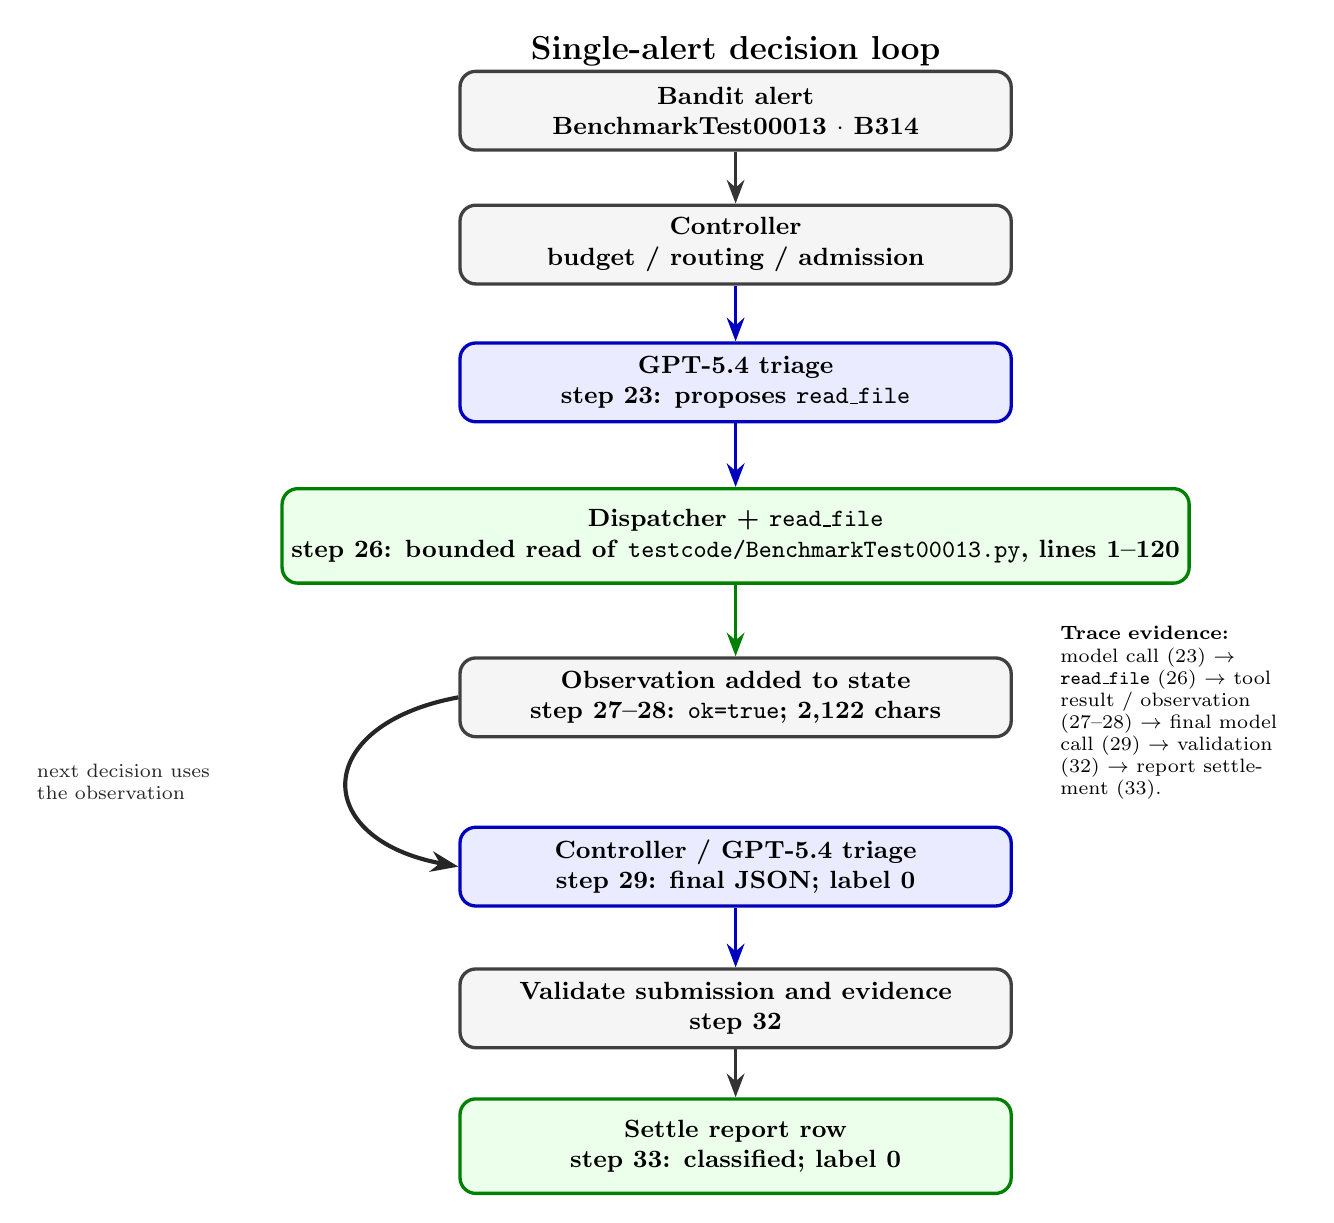
\begin{tikzpicture}[
  >=Stealth,
  runtime/.style={draw=black!75, fill=black!4, rounded corners=2mm, very thick,
    minimum width=7cm, minimum height=10mm, align=center, font=\small\bfseries},
  model/.style={draw=blue!75!black, fill=blue!8, rounded corners=2mm, very thick,
    minimum width=7cm, minimum height=10mm, align=center, font=\small\bfseries},
  tool/.style={draw=green!50!black, fill=green!8, rounded corners=2mm, very thick,
    minimum width=7cm, minimum height=12mm, align=center, font=\small\bfseries},
  runtimearrow/.style={-{Stealth[length=3mm]}, black!80, very thick},
  modelarrow/.style={-{Stealth[length=3mm]}, blue!75!black, very thick},
  toolarrow/.style={-{Stealth[length=3mm]}, green!50!black, very thick},
  loop/.style={-{Stealth[length=3.5mm]}, black!85, line width=1.5pt},
  note/.style={font=\scriptsize, align=left, text width=3.6cm}
]
\node[font=\large\bfseries] at (0,.75) {Single-alert decision loop};
\node[runtime] (alert) at (0,0) {Bandit alert\\BenchmarkTest00013 $\cdot$ B314};
\node[runtime] (controller) at (0,-1.7) {Controller\\budget / routing / admission};
\node[model] (triage) at (0,-3.45) {GPT-5.4 triage\\step 23: proposes \texttt{read\_file}};
\node[tool] (read) at (0,-5.4) {Dispatcher + \texttt{read\_file}\\step 26: bounded read of \texttt{testcode/BenchmarkTest00013.py}, lines 1--120};
\node[runtime] (observation) at (0,-7.45) {Observation added to state\\step 27--28: \texttt{ok=true}; 2,122 chars};
\node[model] (decision) at (0,-9.6) {Controller / GPT-5.4 triage\\step 29: final JSON; label 0};
\node[runtime] (validation) at (0,-11.4) {Validate submission and evidence\\step 32};
\node[tool] (settle) at (0,-13.15) {Settle report row\\step 33: classified; label 0};

\draw[runtimearrow] (alert) -- (controller);
\draw[modelarrow] (controller) -- (triage);
\draw[modelarrow] (triage) -- (read);
\draw[toolarrow] (read) -- (observation);
\draw[loop] (observation.west) .. controls (-5.4,-7.8) and (-5.4,-9.25) ..
  node[note, left, xshift=-2mm] {next decision uses\\the observation} (decision.west);
\draw[modelarrow] (decision) -- (validation);
\draw[runtimearrow] (validation) -- (settle);

\node[note, text width=3cm, anchor=west] at (4,-7.65) {\textbf{Trace evidence:} model call (23) $\rightarrow$ \texttt{read\_file} (26) $\rightarrow$ tool result / observation (27--28) $\rightarrow$ final model call (29) $\rightarrow$ validation (32) $\rightarrow$ report settlement (33).};
\end{tikzpicture}
\end{center}
\noindent\textbf{Figure C2.} Trace-derived decision loop for one successful OWASP alert. The controller routes the model's bounded file-read proposal through the dispatcher; the returned observation changes the next decision, which submits a validated label-0 report row.\\ Source: updated OWASP full-run \texttt{trace(7).jsonl}, steps 23--33.

\clearpage
\subsection*{C3. Limitations and alternatives}

\paragraph{HW1 agent versus plan-and-execute:}
The HW1 agent lets the model choose the next allowed tool call after each observation. A plan-and-execute agent would instead keep an explicit plan in state, carry out planned steps, and revise the plan when new evidence changes the situation. Planning makes progress and the intended work clearer for a long investigation with dependent steps, but it adds planning and revision work, increasing cost and latency. It also needs rules that distinguish a temporary tool failure from a reason to revise the plan. For the Figure C2 alert, one bounded read gave enough evidence for the next model call to submit a result, so a full plan would add more machinery than necessary.

\paragraph{HW1 agent versus supervisor/worker:}
The HW1 agent uses one model and the same three bounded investigation tools for every alert. A supervisor/worker design would add a supervisor that routes the alert to a specialist worker and then receives that worker's result. This can help when different alert types need genuinely different expertise, but it adds a routing call and a worker call, increasing cost and latency. It also requires clear rules for what context passes to each worker and who owns the returned result. A bad routing decision can send an alert to the wrong worker without being noticed. Because the HW1 agent uses the same tools for every alert, separate specialist workers would add overhead without a clear benefit.

\end{document}
